%TODO Why is the global status relevant
%Is there other things that should be described in the report

\section{State Machine}
The watchdog manager has a state machine, shown in
figure~\ref{FIG:GLOBALSTATUSES}. Its transitions depend on the changes of the
global variables, and the current state. If the behavior of the watchdog manager
is correct and the manager is activated, it will stay in the state
'WDGM\_GLOBAL\_STATUS\_OK'. There are however lots of reasons for that the
status will change from the correct state. It depends on the arguments of the
API calls but also the order of the commands that are called and which AUTOSAR
configuration that is supplied. The configuration is important because it
specifies the tolerance of faulty behavior the watchdog should have. It could
also indirectly disable some states and state transition or make some transition
more likely to happen. The effect can for instance come from the number of
checkpoints supplied in the configuration. A correct behavior of the watchdog
manager depends on that checkpoints are reached and does so in the right order
and right timing.

Besides the transition between the deactivated and the OK states, the only
function that can give rise to state transitions for the global status, is the
main function. In an working ECU, the main function should continuously be
called, in a given time interval, by the run time environment (RTE). Note that
the timing is not used when using QuickCheck, see section \ref{SEC:CALLING_COMMANDS}.

\begin{figure}[h!]
  \begin{center}
    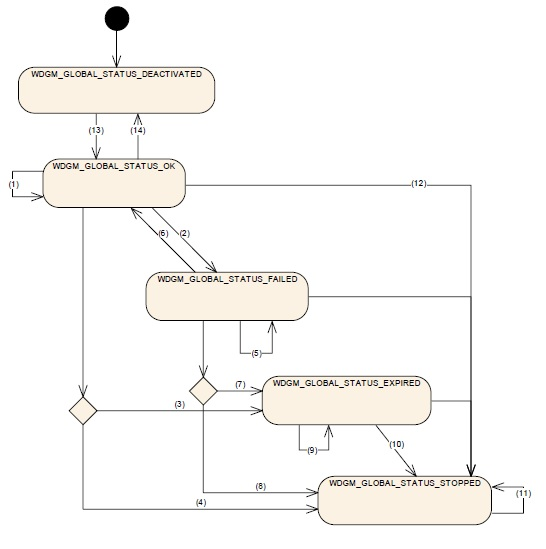
\includegraphics{pictures/globalstatuses.jpg}
  \end{center}
  \caption{State diagram that shows possible trasitions between states}
  \label{FIG:GLOBALSTATUSES}
\end{figure}

\section{Configurations}
The WdgM was tested using three different configurations.
% Which are they and why were they chosen

\subsection{BSI}
A highly simplified configuration \emph{BSI} gives in some sense good results.
Using this configuration the WdgM was never hitting the absorbing state
according to figure \ref{FIG:GLOBALSTATUSES}.  However looking at the state
transitions, comparing figure \ref{FIG:GLOBALSTATUSES} and table
\ref{TABLE:STATUSES_BSI}, only two states are hit. This happens
because the configuration is to simply, it is actually impossible to hit
any other states then \emph{'GLOBAL\_STATUS\_OK'} or
\emph{'GLOBAL\_STATUS\_DEACTIVATED'}. There are no checkpoints or supervision
algorithms configured for the \emph{BSI} configuration.
Hence it is easy to run tests using this configuration but it does, by it self,
not fully test the code because some specification requirements will never be
tested. The untested requirements are mainly requirements for supervision algorithms
that are, according to the configuration, never supposed to be run. Those
untested requirements leaves also other requirements untested because
the watchdog manager never reaches a state when those other requirements must hold.
\begin{figure}[h!]
  \begin{center}
    \subfigure[Shows percentage of each possible command executed]{
      \label{FIG:COMMANDS_BSI}
      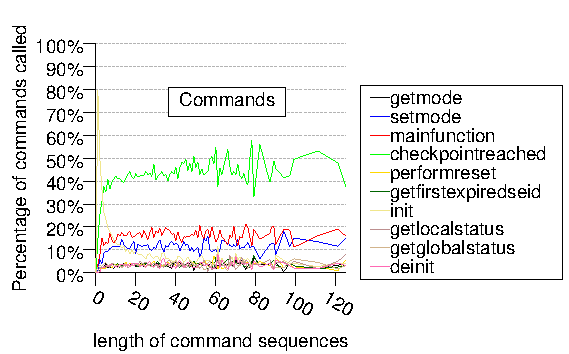
\includegraphics{generated_pictures/history_commands_bsi.pdf}
    }

    \subfigure[Shows percentage of each possible global status hit]{
      \label{FIG:STATUSES_BSI}
      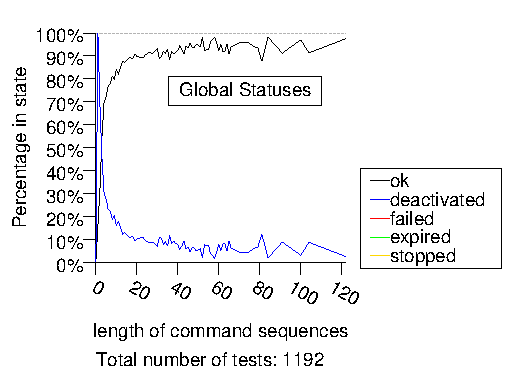
\includegraphics{generated_pictures/history_statuses_bsi.pdf}
    }
  \end{center}
  \caption{BSI configuration}
  \label{FIG:BSI}
\end{figure}

\begin{table}[h!]
  \caption{bsi configuration}
  \label{TABLE:STATUSES_BSI}
  
    \begin{tabular}{r|ccccc}
        \hline
        \multicolumn{6}{c}{Number of tests: 2850} \\
        \hline
        \backslashbox{From}{To}
                    & DEACTIVATED & EXPIRED & FAILED & OK & STOPPED \\
        \hline
        DEACTIVATED & \bf{02.23}\% & 00.00\%       & 00.00\%       & \bf{09.12}\% & 00.00\% \\
        EXPIRED     & 00.00\%       & \bf{00.00}\% & 00.00\%       & 00.00\%       & \bf{00.00}\% \\
        FAILED      & 00.00\%       & \bf{00.00}\% & \bf{00.00}\% & \bf{00.00}\% & \bf{00.00}\% \\
        OK          & \bf{03.24}\% & \bf{00.00}\% & \bf{00.00}\% & \bf{85.41}\% & \bf{00.00}\% \\
        STOPPED     & 00.00\%       & 00.00\%       & 00.00\%       & 00.00\%       & \bf{00.00}\%
      \end{tabular}
    

\end{table}

\subsection{freescale}
The freescale configuration is, compared to BSI, a more realistic configuration.
All supervision algorithms are configured and there are both external and
internal graphs for logical supervision. It is also the configuration, mainly
used at Mecel. The state machine for the global status is totally covered by
running QuickCheck, see table \ref{TABLE:STATUSES_FREESCALE} and figure
\ref{FIG:GLOBALSTATUSES}.


\begin{figure}[h!]
  \begin{center}
    \subfigure[Shows percentage of each possible command executed]{
      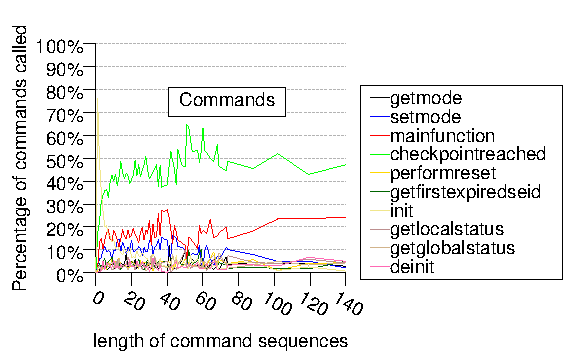
\includegraphics{generated_pictures/history_commands_freescale.pdf}
      \label{FIG:COMMANDS_FREESCALE}
    }
    \subfigure[Shows percentage of each possible global status hit]{
      \label{FIG:STATUSES_FREESCALE}
      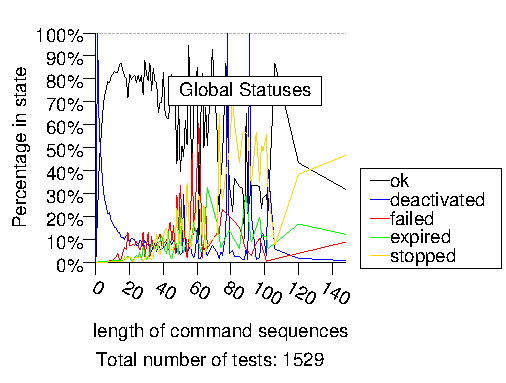
\includegraphics{generated_pictures/history_statuses_freescale.pdf}
    }
  \end{center}
  \caption{Freescale configuration}
  \label{FIG:FREESCALE}
\end{figure}

\begin{table}[!h]
  \caption{Freescale configuration}
  \label{TABLE:STATUSES_FREESCALE}
  
    \begin{tabular}{r|ccccc}
        \hline
        \multicolumn{6}{c}{Number of tests: 1023} \\
        \hline
        \backslashbox{From}{To}
                    & DEACTIVATED & EXPIRED & FAILED & OK & STOPPED \\
        \hline
        DEACTIVATED & \bf{02.43}\% & 00.00\%       & 00.00\%       & \bf{08.32}\% & 00.00\% \\
        EXPIRED     & 00.00\%       & \bf{03.36}\% & 00.00\%       & 00.00\%       & \bf{00.11}\% \\
        FAILED      & 00.00\%       & \bf{00.17}\% & \bf{07.77}\% & \bf{00.12}\% & \bf{00.11}\% \\
        OK          & \bf{02.56}\% & \bf{00.18}\% & \bf{00.87}\% & \bf{69.53}\% & \bf{00.12}\% \\
        STOPPED     & 00.00\%       & 00.00\%       & 00.00\%       & 00.00\%       & \bf{04.34}\%
      \end{tabular}
    

\end{table}

\subsection{example}

\begin{figure}[h!]
  \begin{center}
    \subfigure[Shows percentage of each possible command executed]{
      \label{FIG:COMMANDS_EXAMPLE}
      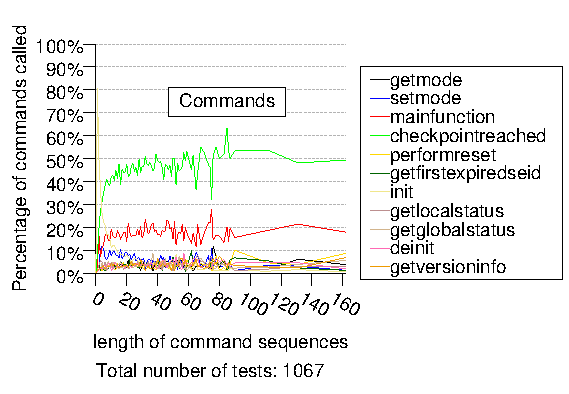
\includegraphics{generated_pictures/history_commands_example.pdf}
    }

    \subfigure[Shows percentage of each possible global status hit]{
      \label{FIG:STATUSES_EXAMPLE}
      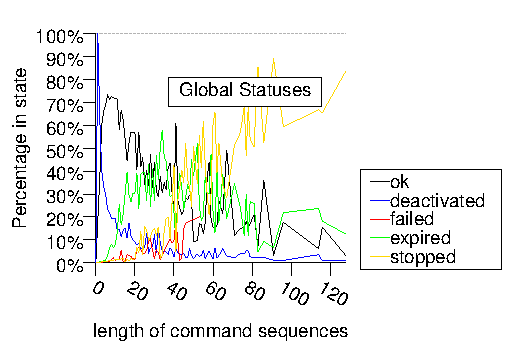
\includegraphics{generated_pictures/history_statuses_example.pdf}
    }
  \end{center}
  \caption{Example configuration}
  \label{FIG:EXAMPLE}
\end{figure}

\begin{table}[!h]
  \caption{example configuration}
  \label{TABLE:STATUSES_EXAMPLE}
  
    \begin{tabular}{r|ccccc}
        \hline
        \multicolumn{6}{c}{Number of tests: 3877} \\
        \hline
        \backslashbox{From}{To}
                    & DEACTIVATED & EXPIRED & FAILED & OK & STOPPED \\
        \hline
        DEACTIVATED & \bf{02.59}\% & 00.00\%       & 00.00\%       & \bf{07.81}\% & 00.00\% \\
        EXPIRED     & 00.00\%       & \bf{24.77}\% & 00.00\%       & 00.00\%       & \bf{00.81}\% \\
        FAILED      & 00.00\%       & \bf{00.12}\% & \bf{02.87}\% & \bf{00.00}\% & \bf{00.04}\% \\
        OK          & \bf{01.68}\% & \bf{02.50}\% & \bf{00.39}\% & \bf{40.22}\% & \bf{00.14}\% \\
        STOPPED     & 00.00\%       & 00.00\%       & 00.00\%       & 00.00\%       & \bf{16.07}\%
      \end{tabular}
    

\end{table}

\section{Handle bugs in the C code}
\label{sec:handlebugs}

\section{Functional safety analysis}
\subsection{Definition of time}
\label{SEC:FUNCTIONAL_SAFETY_TIME}

\section{Statistics}

\section{Functional safety analysis}
Since one important part of the functional safety concept is that it must be
taken in consideration during the hole development process, one can not simply
say that QuickCheck makes it possible to acquire functional safety. There must
first be a number of assumptions. Not even if it is assumed that
every step in the development, until the actual implementation of the watchdog
manager, satisfies the requirements one also has to assume that the remaining
part of the development, towards a finished vehicle, follows the same
constrains. Even further, if this is assumed, there is one important
assumption left before
one can even reason about how QuickCheck can benefit.
This assumptions lies in that the model for the watchdog
manager is correct, namely the AUTOSAR specification.
